\chapter{More Coulomb Energies Dependence Figures}

\begin{figure}[h]
	\begin{center}
		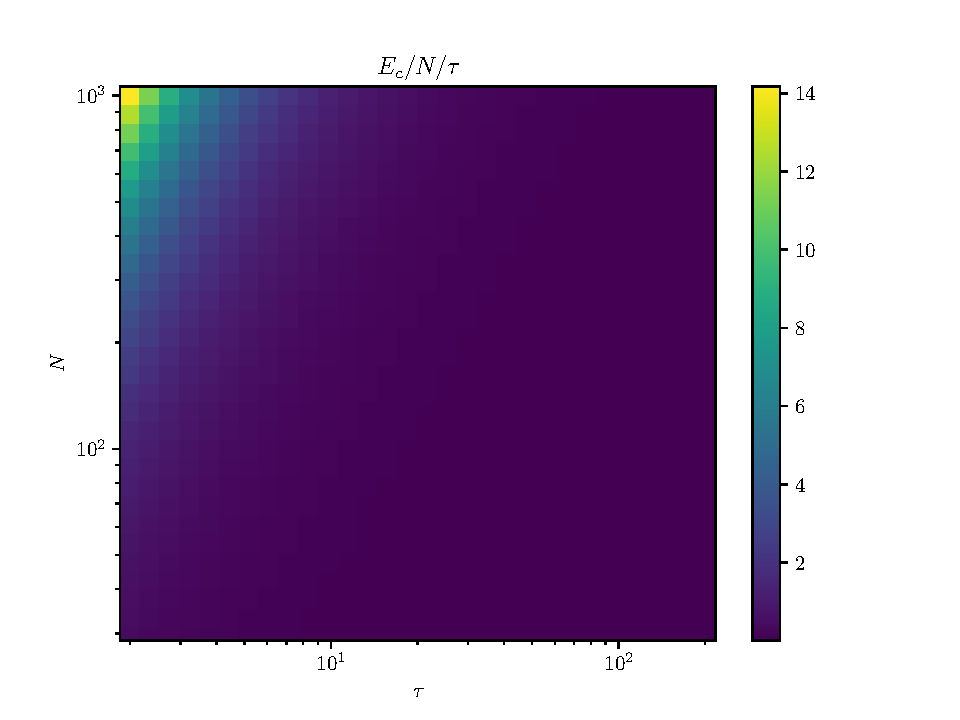
\includegraphics[width=0.9\textwidth]{graphics/coulomb_energy_example@relative_coulomb_energy.pdf}
	\end{center}
	\caption{Same as figure \ref{fig:coulomb_energy}, but with a normalization to $\tau$. Added here to show how $E_c/N$ can exceed $\tau$ for some values of $(\tau,N)$.}
	\label{fig:coulomb_energy_normalized}
\end{figure}

\begin{figure}
	\begin{center}
		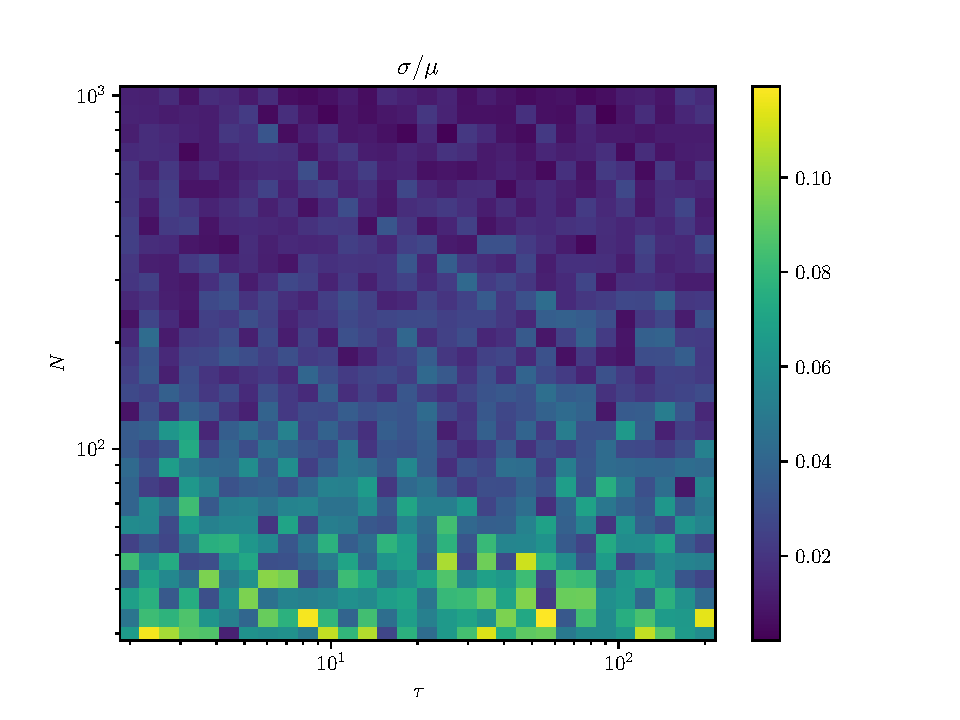
\includegraphics[width=0.85\textwidth]{graphics/coulomb_energy_example@relative_std.pdf}
	\end{center}
	\caption{The relative standard deviation received when generating figure \ref{fig:coulomb_energy}. Naturally, in low $N$ (low-densities), the randomness is larger.}
	\label{fig:coulomb_energy_std}
\end{figure}

\begin{figure}
	\begin{center}
		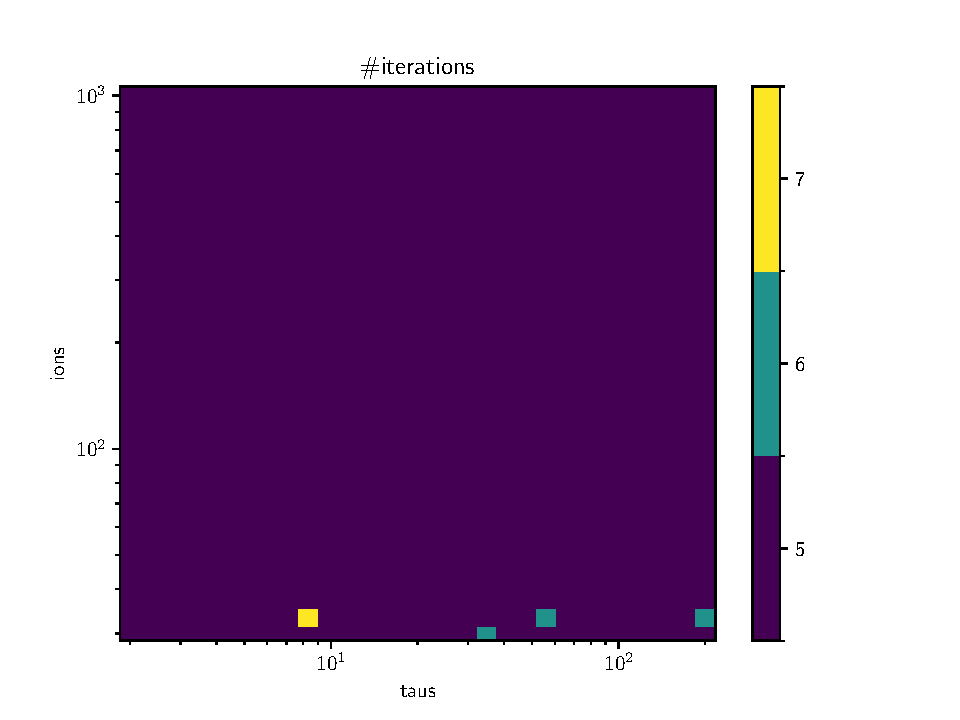
\includegraphics[width=0.85\textwidth]{graphics/coulomb_energy_example@iterations.pdf}
	\end{center}
	\caption{The number of iterations that had to be performed to generate each point in figures \ref{fig:coulomb_energy}. Almost always 5 random number generations is enough to reach a relative standard deviation smaller then $0.12$, however sometimes a few more iterations are needed, naturally for small $N$ (low densities).}
	\label{fig:coulomb_energy_iterations}
\end{figure}
